%!TEX TS-program = xelatex
\documentclass[]{friggeri-cv}
\usepackage{afterpage}
\usepackage{hyperref}
\usepackage{color}
\usepackage{xcolor}
\usepackage{smartdiagram}
\usepackage{fontspec}
% if you want to add fontawesome package
% you need to compile the tex file with LuaLaTeX
% References:
%   http://texdoc.net/texmf-dist/doc/latex/fontawesome/fontawesome.pdf
%   https://www.ctan.org/tex-archive/fonts/fontawesome?lang=en
%\usepackage{fontawesome}
\usepackage{metalogo}
\usepackage{dtklogos}
\usepackage[utf8]{inputenc}
\usepackage{tikz}
\usetikzlibrary{mindmap,shadows}
\hypersetup{
    pdftitle={},
    pdfauthor={},
    pdfsubject={},
    pdfkeywords={},
    colorlinks=false,           % no lik border color
    allbordercolors=white       % white border color for all
}
\smartdiagramset{
    bubble center node font = \footnotesize,
    bubble node font = \footnotesize,
    % specifies the minimum size of the bubble center node
    bubble center node size = 0.5cm,
    %  specifies the minimum size of the bubbles
    bubble node size = 0.5cm,
    % specifies which is the distance among the bubble center node and the other bubbles
    distance center/other bubbles = 0.3cm,
    % sets the distance from the text to the border of the bubble center node
    distance text center bubble = 0.5cm,
    % set center bubble color
    bubble center node color = pblue,
    % define the list of colors usable in the diagram
    set color list = {lightgray, materialcyan, orange, green, materialorange, materialteal, materialamber, materialindigo, materialgreen, materiallime},
    % sets the opacity at which the bubbles are shown
    bubble fill opacity = 0.6,
    % sets the opacity at which the bubble text is shown
    bubble text opacity = 0.5,
}

\addbibresource{bibliography.bib}
\RequirePackage{xcolor}
\definecolor{pblue}{HTML}{0395DE}

\begin{document}
  \vspace{1cm}
\header{Alcemir}{~R. Santos}
      {Software Engineer}
      
% Fake text to add separator      
\fcolorbox{white}{gray}{\parbox{\dimexpr\textwidth-2\fboxsep-2\fboxrule}{%
.....
}}

% In the aside, each new line forces a line break
\begin{aside}
  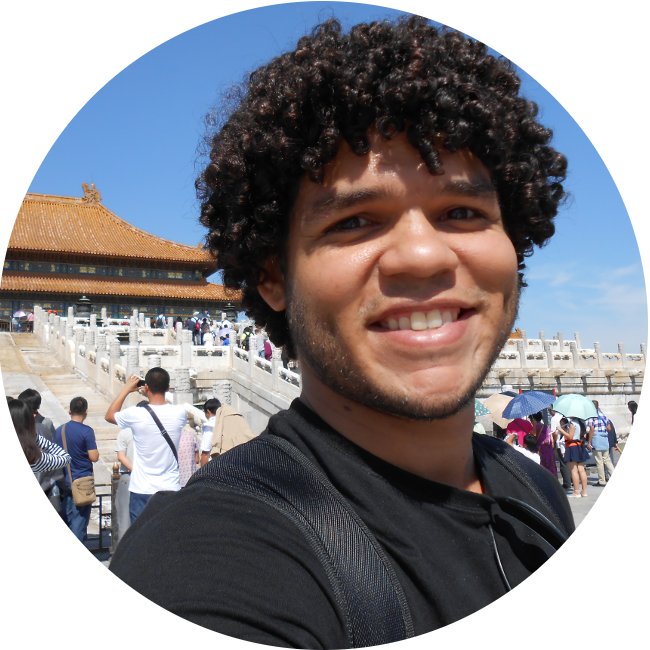
\includegraphics[scale=0.18]{img/eu-circle.png}
  \section{Address}
    Teresina
    Piauí, Brazil
    ~
  \section{Tel \& Skype}
    +55 71  99213 9611
    alcemir\_santos
    ~
  \section{Mail}
    \href{mailto:alcemir.santos@gmail.com}{\textbf{alcemir.santos@}\\gmail.com}
    ~
  \section{Web \& Git}
    \href{http://alcemirsantos.com}{alcemirsantos.com}
    \href{https://bitbucket.org/alcemirsantos}{bitbucket/alcemirsantos}
        \href{https://github.com/alcemirsantos}{github/alcemirsantos}
    ~
  % use  \hspace{} or \vspace{} to change bubble size, if needed
  \section{Programming}
    \smartdiagram[bubble diagram]{
        \textbf{Java},
        \textbf{\vspace{2mm}Python\vspace{2mm}},
        \textbf{Objective C},
        \textbf{C/C++},
        \textbf{R},
        \textbf{PHP}
    }
    ~
  \section{Personal Skills}
    \smartdiagram[bubble diagram]{
        \textbf{Team}\\\textbf{Player},
        \textbf{Initiative},
        \textbf{Curiosity},
        \textbf{Problem}\\\textbf{Solving},
        \textbf{\vspace{2mm}Manage\vspace{2mm}},
        \textbf{Organize}
    }
    ~
\end{aside}
~
\section{Education}
\begin{entrylist}
     \entry
     {2014 - 2017?}
     {Ph.D in Computer Science}
     {Federal University of Bahia}
     {4 years scholarship grant from FAPESB.\\}
    \entry
    {2011 - 2013}
    {Master's Degree in Computer Science}
    {Federal University of Minas Gerais}
    {2 years scholarship grant from CNPq.\\}
    \entry
    {2006 - 2010}
    {Bachelor's Degree in Computer Science}
    {Federal University of Piauí}
    {2$^{nd}$ Best grade among the classmates.\\}
    \entry
    {2003 - 2005}
    {High School Diploma}
    {CEBRAPI}
    {3$^{rd}$ Best grade among the classmates.}
\end{entrylist}
\\
\section{Experience}
\begin{entrylist}
    \entry
    {2015 - 2016}
    {Ph.D. Visiting Student}
    {Universit\"at Passau}
    {I lived on year in Passau. During this time I had to work together with other \textit{Ph.D.} students from the local University research group under supervision of Prof. Sven Apel. Among my responsabilities were to build a tool for collecting software repositories metadata about conflict merges and built developer networks from them. Most of the time I programmed with \texttt{Java}, but also learned some \texttt{Python} and \texttt{R}. \\}
  \entry
    {2013 - 2014}
    {Software Engineering Research Assistent}
    {Reuse in Software Engineering Laboratory (RiSE Labs)}
    {During one year I had to work together with the \textit{Master} and \textit{Ph.D.} students from the research group. Among my responsabilities were to help the students with the design and execution of software engineering experiments in different Software Engineering topics, as well as sofware development and testing with \texttt{Java} and \texttt{Objective-C}. \\}
  \entry
    {01/2010-02/2011}
    {Web Developer}
    {Freelance}
    {Just prior to finish my CS Degree I have worked as Full-Stack Freelance Web-developer in small projects for local events and our local Judo team with \texttt{PHP}.\\}
    \entry
    {2008 - 2009}
    {Research Internship}
    {Federal University of Piauí}
    {During one year I have programmed neural networks addressing interger optimization problems mainly using SciLab.}
   
\end{entrylist}



\newpage

\begin{aside}
~
~
~
  \section{OS Preference}
    \textbf{GNU/Linux}
\includegraphics[scale=0.40]{img/5stars.png}
    \textbf{MacOS}
\includegraphics[scale=0.40]{img/4stars.png}
    \textbf{Windows}
\includegraphics[scale=0.40]{img/1stars.png}
    ~
  \section{Places Lived}
    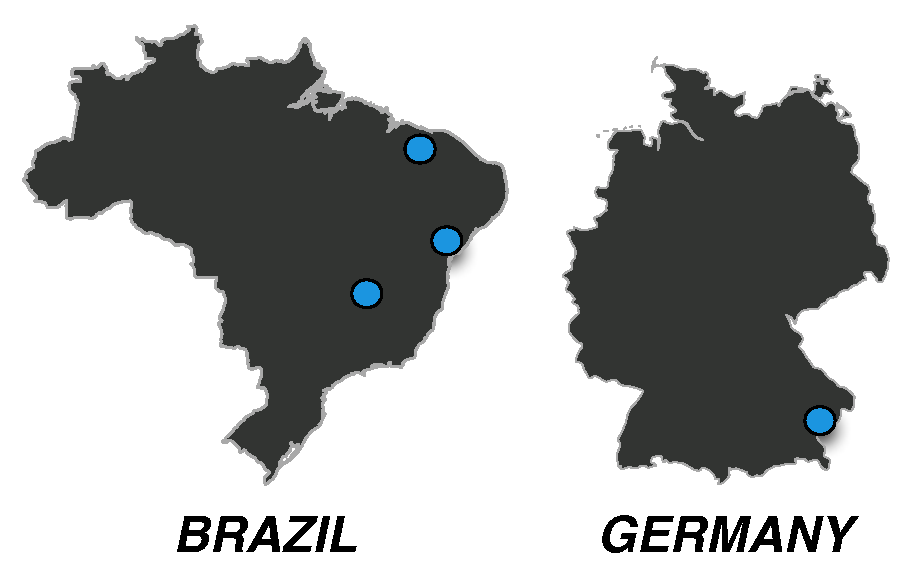
\includegraphics[scale=0.25]{img/places.pdf}
    ~
  \section{Languages}
    \textbf{Portuguese}
\includegraphics[scale=0.40]{img/5stars.png}
    \textbf{English}
\includegraphics[scale=0.40]{img/4stars.png}
    \textbf{German}
\includegraphics[scale=0.40]{img/3stars.png}
    \textbf{Spanish}
\includegraphics[scale=0.40]{img/1stars.png}
    ~
\end{aside}

\section{Publications}
Author, Author, Author\\
\textbf{Lorem ipsum dolor sit amet, consectetur adipiscing elit, sed do eiusmod tempor incididunt ut labore et dolore magna aliqua}\\
\emph{Lorem ipsum dolor sit amet, consectetur adipiscing elit, sed do eiusmod tempor incididunt ut labore et dolore magna aliqua}
\\
\section{Honors \& Awards}
\begin{entrylist}
  \entry
    {10/2015}
    {Best swordsman duel}
    {Contest}
    {Lorem ipsum.\\
    \emph{Lorem ipsum}}
\end{entrylist}

\section{Certifications}
\begin{entrylist}
  \entry
    {02/2013}
    {Intro to Computer Science}
    {Udacity. E-learning}
    {\emph{Building a Python Search Engine}}
\end{entrylist}

\section{Other Info}
For the Italian job market:\\
\emph{Si autorizza il trattamento delle informazioni contenute nel curriculum in conformità alle disposizioni previste dal d.lgs. 196/2003. Si dichiara altresì di essere consapevole che, in caso di dichiarazioni non veritiere, si è passibili di sanzioni penali ai sensi del DPR 445/00 oltre alla revoca dei benefici eventualmente percepiti.}
\\
\begin{flushleft}
\emph{May 8th, 2016}
\end{flushleft}
\begin{flushright}
\emph{John Snow}
\end{flushright}

\end{document}
